\documentclass[10pt,a4paper]{article}
\usepackage[utf8]{inputenc} % para poder usar tildes en archivos UTF-8
\usepackage[spanish]{babel} % para que comandos como \today den el resultado en castellano
\usepackage{a4wide} % márgenes un poco más anchos que lo usual
\usepackage[conEntregas]{caratula}
\usepackage{hyperref} % para hipervínculos
\usepackage{amsmath} % para matemática en varias lineas
\usepackage{synttree} % para arboles de derivación
\usepackage{graphicx} %imágenes
\usepackage{float}
\usepackage{color}
\graphicspath{ {../Resultados/} }


\begin{document}

\titulo{Trabajo Práctico}
\subtitulo{Parser para gramática PEGS }

\fecha{\today}

\materia{Teoría de Lenguajes de Programación}
\grupo{Grupo 10}

\integrante{Garbi, Sebastían}{179/05}{garbyseba@gmail.com}
\integrante{Sarries, Ana}{144/02}{anasarries@yahoo.com.ar}
% Pongan cuantos integrantes quieran

\maketitle

\section{Introducción}
Para la realización de este trabajo contamos con las reglas de un lenguaje simple con el cual se pueden generar composiciones visuales complejas con muy pocas lineas de definición. Este trabajo práctico consiste en generar un analizador léxico-sintáctico que pueda interpretar archivos escritos con ese lenguaje y luego darle semántica a lo interpretado generando la composición visual resultante. Para este cometido utilizaremos PLY\footnote{Python Lex Yacc} de Python, y los conocimientos aprendidos en la materia para configurar correctamente dicha herramienta.
\section{Gramática}
Para interpretar el lenguaje se generó la gramática $G = \left<{V_n,V_t,P,Programa}\right>$ donde:
\begin{itemize}
\item $V_n$ es: \{Elemento, Elementoand, Elementobase, Factor, Main, Masreglas, Numero, Prim, Programa, Reglas, Termino, Trans, Unaregla\}
\item $V_t$ es:\{\$, \&, (, ), *, +, -, ., /, :, $<$, =, $>$, BALL, BOX, CB, CG, CR, D, NADA, NUM, REGLA, RX, RY, RZ, S, SX, SY, SZ, TX, TY, TZ, [, ], \^{},$\vert$ \}
\item Producciones P:\\
$Programa\rightarrow{}Reglas\;Main\;Masreglas$\\
$Reglas\rightarrow{}\lambda$\\
$Reglas\rightarrow{}Reglas\;Unaregla$\\
$Main\rightarrow{}\$\;=\;Elemento$\\
$Main\rightarrow{}\$.\;=\;Elemento$\\
$Masreglas\rightarrow{}\lambda$\\
$Masreglas\rightarrow{}Masreglas\;Unaregla$\\
$Masreglas\rightarrow{}Masreglas\;Main$\\
$Unaregla\rightarrow{}\textbf{REGLA}\;=\;Elemento$\\
$Unaregla\rightarrow{}\textbf{REGLA.}\;=\;Elemento$\\
$Elemento\rightarrow{}Elemento\;|\;Elementoand$\\
$Elemento\rightarrow{}Elementoand$\\
$Elementoand\rightarrow{}Elementoand\;\&\;Elementobase$\\
$Elementoand\rightarrow{}Elementobase$\\
$Elementobase\rightarrow{}Prim$\\
$Elementobase\rightarrow{}Elementobase\;:\;Trans$\\
$Elementobase\rightarrow{}[\;Elemento\;]$\\
$Elementobase\rightarrow{}Elementobase\;{}^\wedge\;Numero$\\
$Elementobase\rightarrow{}<\;Elemento\;>$\\
$Elementobase\rightarrow{}\textbf{REGLA}$\\
$Elementobase\rightarrow{}\$$\\
$Prim\rightarrow{}\textbf{BALL}$\\
$Prim\rightarrow{}\textbf{BOX}$\\
$Prim\rightarrow{}\textbf{NADA}$\\
$Trans\rightarrow{}\textbf{RX}\;Numero$\\
$Trans\rightarrow{}\textbf{RY}\;Numero$\\
$Trans\rightarrow{}\textbf{RZ}\;Numero$\\
$Trans\rightarrow{}\textbf{S}\;Numero$\\
$Trans\rightarrow{}\textbf{SX}\;Numero$\\
$Trans\rightarrow{}\textbf{SY}\;Numero$\\
$Trans\rightarrow{}\textbf{SZ}\;Numero$\\
$Trans\rightarrow{}\textbf{TX}\;Numero$\\
$Trans\rightarrow{}\textbf{TY}\;Numero$\\
$Trans\rightarrow{}\textbf{TZ}\;Numero$\\
$Trans\rightarrow{}\textbf{CR}\;Numero$\\
$Trans\rightarrow{}\textbf{CG}\;Numero$\\
$Trans\rightarrow{}\textbf{CB}\;Numero$\\
$Trans\rightarrow{}\textbf{D}\;Numero$\\
$Numero\rightarrow{}Numero\;+\;Factor$\\
$Numero\rightarrow{}Numero\;-\;Factor$\\
$Numero\rightarrow{}Factor$\\
$Factor\rightarrow{}Factor\;*\;Termino$\\
$Factor\rightarrow{}Factor\;/\;Termino$\\
$Factor\rightarrow{}Termino$\\
$Termino\rightarrow{}\textbf{NUM}$\\
$Termino\rightarrow{}+\;\textbf{NUM}$\\
$Termino\rightarrow{}-\;\textbf{NUM}$\\
$Termino\rightarrow{}(\;Numero\;)$\\
$Termino\rightarrow{}+\;(\;Numero\;)$\\
$Termino\rightarrow{}-\;(\;Numero\;)$\\
\end{itemize}
De $V_t$ cabe destacar el token $\textbf{NADA}$ que es el que representa al caractér ``\_'',  el token $\textbf{REGLA}$ que se corresponde con la expresión regular `\lbrack a-zA-Z\rbrack+' y el token $\textbf{NUM}$ con la expresión regular `\textbackslash d+(\textbackslash .\textbackslash d+)?'.\\
Los demás tokens se corresponden literalmente con su texto en minúscula, por ejemplo $BALL$ con la palabra ``ball''.\\
Para que estos últimos no sean tokenizados como $\textbf{REGLA}$ se usó el ejemplo de palabras reservadas que aparece en la sección \textbf{4.3} de la documentación de ply (\url{http://www.dabeaz.com/ply/ply.html#ply_nn6}).\\
Existe también una forma de reconocer comentarios encerrados entre comillas dobles, los cuales serán descartados sin más.

\section{Implementación de la solución}
La solución consiste de dos grandes pasos.\\
El primero ocurre mientras se ejecuta el analizador sintáctico, en este paso se ``sintetiza'' en el \textbf{NT} que generó la producción el objeto que va a ser mostrado así también las transformaciones que sufre el mismo.
Para las producciones donde se define un nombre de regla\footnote{Estamos utilizando que \$ es un nombre de regla}, por ejemplo ``$bola=ball|box$'', utilizamos dos diccionarios globales ``reglas'' y ``finales''. Si la regla no es final se define solo en el diccionario ``reglas'', en cambio si es final (tiene `.') se define en ambos diccionarios.\\
El segundo paso es al momento de mostrar, en este paso se toma del diccionario ``reglas'' la definición de \textbf{\$} y se le ejecuta el método \textbf{mostrar} que se encargará de mostrar todos los elementos que se generaron durante el parseo.\\
\\
Una estado se define con tres atributos: 
\begin{itemize}
\item{\textbf{space}: Consiste de una matriz de 4*4 de la cual se obtendrán los valores para ubicar el elemento en el espacio}
\item{\textbf{color}: Un array de 3 posiciones que representan cada componente de color}
\item{\textbf{depth}: Un entero que representa la máxima cantidad de reemplazos de  reglas de la composición visual}
\end{itemize}
Transformar consiste en mezclar dos de estos estados de manera que el estado resultante sera un producto de matrices para \textbf{space}, un producto elemento a elemento para \textbf{color} y el menor de los \textbf{depth}.\\
De este modo podemos definir estado identidad como:\\
\textbf{space} = $\begin{bmatrix}
1 & 0 & 0 & 0\\ 
0 & 1 & 0 & 0\\ 
0 & 0 & 1 & 0\\ 
0 & 0 & 0 & 1\\
\end{bmatrix}$\\
\textbf{color} = $\begin{bmatrix}1, 1 ,1\end{bmatrix}$\\
\textbf{depth} = 100\\
\\
 Para la solución se crearon dos jerarquías de clases que interactúan entre sí. Una es la que se refiere a las transformaciones:\\
De Transformacion heredan TransRX, TransRY, TransRZ, TransT, TransS, TransC, TransD, cada una de ellas representa un tipo de transformación según su nombre lo indica.\\
Cada transformación es un estado que al aplicarse a otro lo afecta de la manera deseada.\\
A su vez las instancias directas de Transformacion se corresponde con la transformación identidad, la cual al ser aplicada no efectúa ningún cambio. Ésta es el estado inicial de todo elemento.\\
La otra jerarquía es la de Elementos:
De Elemento heredan Primitiva, Compuesta, ElementoPOT, ElementoCorchete y ElementoREGLA. De Primitiva heredan Ball, Box y Nada, y de Compuesta heredan ElementoOR, ElementoAND y  ElementoANDTransformaDirecto.\\
Las clases del subárbol de Primitiva representan cada una un objeto final que se mostrará en la composición visual final.\\
Las clases del subárbol de Compuesta implementan un patrón ``composite'' los cuales reenviaran a sus contenidos los mensajes que reciban.\\
Las clases ElementoCorchete y ElementoPOT también siguen este patrón pero conteniendo un solo elemento.\\
La clase ElementoCorchete tiene mensajes especiales para interactuar con ElementoPOT, en caso de que ésta última lo contenga, en otro caso simplemente reenvía los mensajes a su elemento contenido.\\
Todos los Elementos tienen implementados los métodos para interactuar con ElementoPOT de forma tal que éste los repita sin el comportamiento especial que tiene ElementoCorchete.\\
Gracias a la forma en que está hecha la gramática, las precedencias están resueltas al momento del parseo, con lo cual, podemos ir creando los objetos a medida que el parser va interpretando el archivo.\\
\textbf{ElementoOR} representa una cadena de $|$, por ejemplo $A|B|C|D$ donde A, B, C, D puede ser cualquier elemento.
Las producciones que parten del NT Elemento crean éste tipo de elemento de la siguiente manera:\\
$Elemento\rightarrow{}Elementoand$\\
$\{Elemento.valor \Leftarrow{} ElementoOR().append(Elementoand.valor\}$\\
$Elemento\rightarrow{}Elemento_{1}\;|\;Elementoand$\\
\{$Elemento.valor \Leftarrow{}Elemento_{1}.valor.append(Elementoand.valor)\}$\\
Analogamente \textbf{ElementoAND} representa una cadena $A\&B\&C\&D$ y se creasiguiendo las mismas reglas.\\
\textbf{ElementoRegla} se crea instanciando  con referencias a los diccionarios ``reglas'' y ``finales' para las producciones:\\
$Elementobase\rightarrow{}\textbf{REGLA}$\\
$Elementobase\rightarrow{}\$$\\
\textbf{ElementoPOT} y  \textbf{ElementoCorchete} se crean respectivamente con las producciones:\\
$Elementobase\rightarrow{}Elementobase\;{}^\wedge\;Numero$\\
$Elementobase\rightarrow{}[\;Elemento\;]$\\
Con la produccion ``$Elementobase\rightarrow{}<\;Elemento\;>$''
se crea una instancia de \textbf{ElementoOR} donde se agrega el elemento junto con un elemento primitivo \textbf{Nada} para que tenga 50\% de probabilidades de aparecer

Teniendo en cuenta que puede haber más de una definición del mismo nombre de regla y que esto es equivalente a tener un `\textbar' entre las dos definiciones, todas las definiciones del diccionario reglas son \textbf{ElementoOR} al cual se van agregando las nuevas definiciones, teniendo así un único valor para la misma clave el cual se encargara de decidir cual de las definiciones aplicar\footnote{Al ser tratada cada definición como Elementos diferentes, ésto no afecta a los `\textbar' internos de cada definición}.\\
\begin{align}
\left.\begin{matrix}Reg = A\\
Reg = B\\
\end{matrix}\right\} \equiv Reg = A|B
\end{align}
\\
Los elementos tienen estados inicializados con la transformación identidad. Cada vez que reciben una transformación se modifica dicho estado.\\
Los estados tienen 2 mensajes principales: \textit{transformar} que dada una Trasnformacion transforma su estado interno y \textit{mostrar} que define las reglas de como se muestra el Elemento en la composición visual. Por ejemplo al mandarle el mensaje \textit{mostrar} a un \textbf{ElementoOR}, éste tomará pseudo-aleatoriamente uno de sus elementos contenidos y le enviará el mensaje \textit{mostrar}
\section{Arboles de derivación}
En esta sección se van a presentar algunos ejemplos parseados junto con los arboles de derivación que genera cada entrada.\\
\begin{itemize}
\item{$\$=box$\\
\synttree
[Programa
	[Reglas [ $\lambda$] ]
	[Main
		[\$]
		[=]
		[Elemento
			[Elementoand
				[Elementobase
					[Prim [BOX] ]
				]
			]
		]
	]
	[Masreglas [ $\lambda$] ]
]
}
\item{$\$=ball\&box:tx1$\\
\synttree
[Programa
	[Reglas [ $\lambda$] ]
	[Main [\$] [=]
		[Elmento [Elementoand [Elementoand [Elementobase [Prim [BALL]]]][\&] [Elementobase [Elementobase [Prim [BOX]]] [ : ] [Trans [TX] [Numero [Factor [Termino [NUM] ] ] ]]]]]]
	[Masreglas [ $\lambda$] ]
]}
\pagebreak
\item{$A=ball$\\
$\$=A|B|\_$\\
$B=box$\\
\synttree
[Programa[Reglas*1][Main[\$][=][Elemento[Elemento[Elemento[Elementoand[Elementobase[REGLA]]]][\textbar][Elementoand[Elementobase[REGLA]]]][\textbar][Elementoand[Elementobase[Prim [NADA]]]]]][Masreglas*2]]\\
\synttree
[Reglas*1[Reglas[$\lambda$]][Unaregla[REGLA][=][Elemento[Elementoand[Elementobase[Prim[BALL]]]]]]]
\synttree
[Masreglas*2[Masreglas[$\lambda$]][Unaregla[REGLA][=][Elemento[Elementoand[Elementobase[Prim[BOX]]]]]]]
}
\end{itemize}

En el directorio Derivaciones se puede encontrar las listas de producciones utilizadas para generar cada uno de los ejemplos del directorio TL2014C2-TP-Ejemplos. Estas listas conforman las derivaciones mas a la derecha invertidas generadas por el parser LALR

\section{Algunos resultados}
\subsection{Resultados válidos}
\begin{figure}[H]
\centering
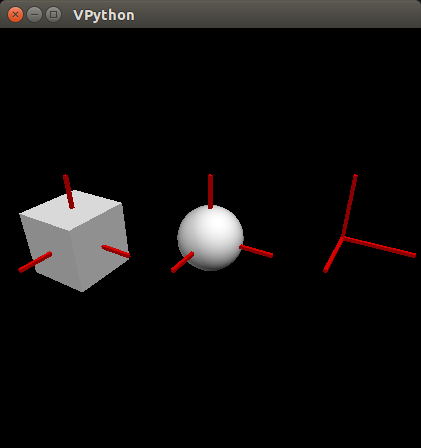
\includegraphics[scale=0.3]{eg01.png}
\caption{Primitivas eg01.peg}
\end{figure}
\begin{figure}[H]
\centering
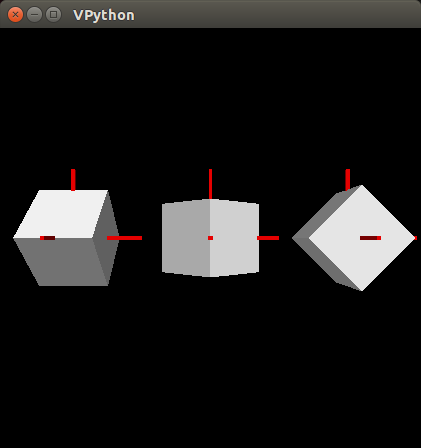
\includegraphics[scale=0.3]{eg02.png}
\caption{Transf. Rotar eg02.peg}
\end{figure}
\begin{figure}[H]
\centering
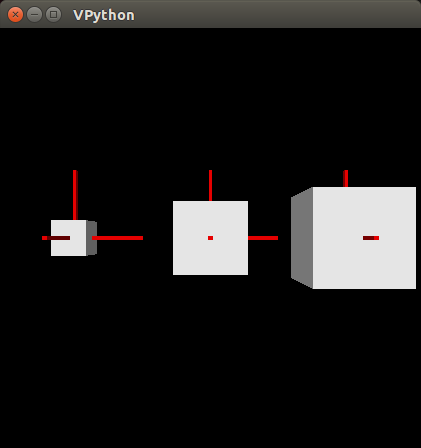
\includegraphics[scale=0.3]{eg03.png}
\caption{Transf. Escala simétrica  eg03.peg}
\end{figure}
\begin{figure}[H]
\centering
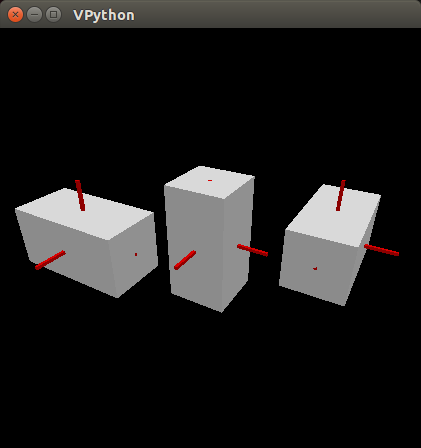
\includegraphics[scale=0.3]{eg04.png}
\caption{Transf. Escala en ejes eg04.peg}
\end{figure}
\begin{figure}[H]
\centering
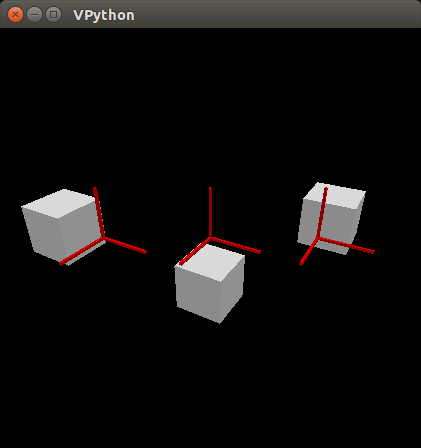
\includegraphics[scale=0.3]{eg05.png}
\caption{Transf. Traslación eg05.peg}
\end{figure}
\begin{figure}[H]
\centering
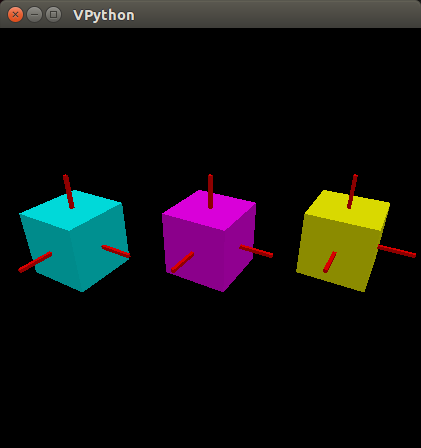
\includegraphics[scale=0.3]{eg06.png}
\caption{Transf. Color eg06.peg}
\end{figure}
\pagebreak


\subsection{Resultados inválidos}
Hay tres tipos de resultados inválidos, de los cuales los dos primeros lanzan una excepción SyntaxError y el último una Exception :
\begin{itemize}
\item Caracteres inválidos en el archivo.\\$\$=A|B\\Regla=ball\%\\A=B|Regla$\\El símbolo ``\%'' no es parte del lenguaje\\
\textcolor{red}{SyntaxError: Caracter ilegal en la linea 2 cerca de '\%\\A=B|Regla\\'}
\item Palabra mal formada.\\$\$=A|B\\Regla55=ball\\A=B|Regla55$\\Si bien el analizador léxico reconoce los números, los nombres de reglas sólo admiten letras mayúsculas y minúsculas.\\
\textcolor{red}{SyntaxError: Error de sintaxis en la linea 2 cerca de '55' reconocido como NUM '55.0'}
\item Otra forma de que el parser falle es si se utiliza alguna regla que no fue definida.\\$\$=A|B\\Regla=ball\\A=B|Regla$\\\$ usa las reglas A y B pero B nunca fue definida.\\
\textcolor{red}{Exception: La regla B no está definida}
\end{itemize}
\section{Ejecución}
El programa debe ser ejecutado de la siguiente manera:\\
$python\;parser.py\;ruta/al/archivo.peg$\\

En el archivo parser.py hay tres variables boolenas globales útiles para mostrar más información:\\
	$mostrarTokens$ Imprime la lista de Tokens que generó el analizador léxico\\
	$mostrarEjes$ Muestra en la composición visual los ejes X(Rojo) Y(Verde) Z(Azul) centrado en el origen desde -5 a +5 en cada eje\\
	$mostrarProducciones$ Muestra la lista de producciones generada por el parser LALR\\
\section{Detalle de requerimientos}
	Para la implementación del trabajo práctico se utilizaron las bibliotecas de Python:
\begin{itemize}
\item sys
\item numpy
\item math
\item copy 
\item visual (VPython)
\item random
\item ply
\item re
\end{itemize}
\section{Desiciones}
Decidimos pensar a \$ como un nombre de regla cualquiera el cual puede estar definido varias veces e incluso puede ser llamado por otra regla; asimismo se le puede definir alguna final con ``\$.''.\\
\\
En las producciones \\
$Elementobase\rightarrow{}Elementobase\;:\;Trans$\\
$Trans\rightarrow{}\textbf{RX}\;Numero$ \\
$Trans\rightarrow{}\textbf{RY}\;Numero$ (Por dar un ejemplo)\\
podríamos haber puesto \\
$Elementobase\rightarrow{}Elementobase\;:\;Trans\;Numero$\\
$Trans\rightarrow{}\textbf{RX}$\\
$Trans\rightarrow{}\textbf{RY}$\\
Decidimos por la primera porque nos permite crear el objeto de transformación instanciado en el mismo paso.\\
\\
Optamos por esa estructura de clases para Elemento porque resultaba más natural delegarle a cada objeto que supiera sus reglas de mostrado y transformación, y la gramática nos dejaba armarlos transformarlos y componerlos fácilmente.
\\
Probamos con otras producciones \\
$Programa\rightarrow{}Reglas\;Main\;Reglas$\\
$Reglas\rightarrow{}\lambda$\\
$Reglas\rightarrow{}Reglas\;Main$\\
$Reglas\rightarrow{}Reglas\;Unaregla$\\
Pero generaba un conflicto Reduce/Reduce yendo por Reglas $\rightarrow$ Main\\
$\left.\begin{matrix}
Programa\rightarrow{}\bullet\;Reglas\;Main\;Reglas\\
Reglas\rightarrow{} \bullet\\
Reglas\rightarrow{} \bullet\;Reglas\;Main\\
\end{matrix}\right\} \xrightarrow{Reglas}
\left.\begin{matrix}
Programa\rightarrow{}Reglas\;\bullet\;Main\;Reglas\\
Reglas\rightarrow{} Reglas\;\bullet\;Main\\
\end{matrix}\right\}\xrightarrow{Main}
\left.\begin{matrix}
Programa\rightarrow{}Reglas\;Main\;\bullet\;Reglas\\
Reglas\rightarrow{} \bullet \\
Reglas\rightarrow{} Reglas\;Main\;\bullet\\
\end{matrix}\right\}$
\section{Conclusión}

\end{document}
